\documentclass[twoside]{book}

% Packages required by doxygen
\usepackage{fixltx2e}
\usepackage{calc}
\usepackage{doxygen}
\usepackage[export]{adjustbox} % also loads graphicx
\usepackage{graphicx}
\usepackage[utf8]{inputenc}
\usepackage{makeidx}
\usepackage{multicol}
\usepackage{multirow}
\PassOptionsToPackage{warn}{textcomp}
\usepackage{textcomp}
\usepackage[nointegrals]{wasysym}
\usepackage[table]{xcolor}

% Font selection
\usepackage[T1]{fontenc}
\usepackage[scaled=.90]{helvet}
\usepackage{courier}
\usepackage{amssymb}
\usepackage{sectsty}
\renewcommand{\familydefault}{\sfdefault}
\allsectionsfont{%
  \fontseries{bc}\selectfont%
  \color{darkgray}%
}
\renewcommand{\DoxyLabelFont}{%
  \fontseries{bc}\selectfont%
  \color{darkgray}%
}
\newcommand{\+}{\discretionary{\mbox{\scriptsize$\hookleftarrow$}}{}{}}

% Page & text layout
\usepackage{geometry}
\geometry{%
  a4paper,%
  top=2.5cm,%
  bottom=2.5cm,%
  left=2.5cm,%
  right=2.5cm%
}
\tolerance=750
\hfuzz=15pt
\hbadness=750
\setlength{\emergencystretch}{15pt}
\setlength{\parindent}{0cm}
\setlength{\parskip}{3ex plus 2ex minus 2ex}
\makeatletter
\renewcommand{\paragraph}{%
  \@startsection{paragraph}{4}{0ex}{-1.0ex}{1.0ex}{%
    \normalfont\normalsize\bfseries\SS@parafont%
  }%
}
\renewcommand{\subparagraph}{%
  \@startsection{subparagraph}{5}{0ex}{-1.0ex}{1.0ex}{%
    \normalfont\normalsize\bfseries\SS@subparafont%
  }%
}
\makeatother

% Headers & footers
\usepackage{fancyhdr}
\pagestyle{fancyplain}
\fancyhead[LE]{\fancyplain{}{\bfseries\thepage}}
\fancyhead[CE]{\fancyplain{}{}}
\fancyhead[RE]{\fancyplain{}{\bfseries\leftmark}}
\fancyhead[LO]{\fancyplain{}{\bfseries\rightmark}}
\fancyhead[CO]{\fancyplain{}{}}
\fancyhead[RO]{\fancyplain{}{\bfseries\thepage}}
\fancyfoot[LE]{\fancyplain{}{}}
\fancyfoot[CE]{\fancyplain{}{}}
\fancyfoot[RE]{\fancyplain{}{\bfseries\scriptsize Generated by Doxygen }}
\fancyfoot[LO]{\fancyplain{}{\bfseries\scriptsize Generated by Doxygen }}
\fancyfoot[CO]{\fancyplain{}{}}
\fancyfoot[RO]{\fancyplain{}{}}
\renewcommand{\footrulewidth}{0.4pt}
\renewcommand{\chaptermark}[1]{%
  \markboth{#1}{}%
}
\renewcommand{\sectionmark}[1]{%
  \markright{\thesection\ #1}%
}

% Indices & bibliography
\usepackage{natbib}
\usepackage[titles]{tocloft}
\setcounter{tocdepth}{3}
\setcounter{secnumdepth}{5}
\makeindex

% Hyperlinks (required, but should be loaded last)
\usepackage{ifpdf}
\ifpdf
  \usepackage[pdftex,pagebackref=true]{hyperref}
\else
  \usepackage[ps2pdf,pagebackref=true]{hyperref}
\fi
\hypersetup{%
  colorlinks=true,%
  linkcolor=blue,%
  citecolor=blue,%
  unicode%
}

% Custom commands
\newcommand{\clearemptydoublepage}{%
  \newpage{\pagestyle{empty}\cleardoublepage}%
}

\usepackage{caption}
\captionsetup{labelsep=space,justification=centering,font={bf},singlelinecheck=off,skip=4pt,position=top}

%===== C O N T E N T S =====

\begin{document}

% Titlepage & ToC
\hypersetup{pageanchor=false,
             bookmarksnumbered=true,
             pdfencoding=unicode
            }
\pagenumbering{alph}
\begin{titlepage}
\vspace*{7cm}
\begin{center}%
{\Large My Project }\\
\vspace*{1cm}
{\large Generated by Doxygen 1.8.12}\\
\end{center}
\end{titlepage}
\clearemptydoublepage
\pagenumbering{roman}
\tableofcontents
\clearemptydoublepage
\pagenumbering{arabic}
\hypersetup{pageanchor=true}

%--- Begin generated contents ---
\chapter{Template}
\label{md__r_e_a_d_m_e}
\hypertarget{md__r_e_a_d_m_e}{}
Visual Studio 2015 Templates 
\chapter{Hierarchical Index}
\section{Class Hierarchy}
This inheritance list is sorted roughly, but not completely, alphabetically\+:\begin{DoxyCompactList}
\item \contentsline{section}{C\+Base4618}{\pageref{class_c_base4618}}{}
\begin{DoxyCompactList}
\item \contentsline{section}{C\+Pong}{\pageref{class_c_pong}}{}
\item \contentsline{section}{C\+Sketch}{\pageref{class_c_sketch}}{}
\end{DoxyCompactList}
\item \contentsline{section}{C\+Control}{\pageref{class_c_control}}{}
\item \contentsline{section}{Client}{\pageref{class_client}}{}
\item \contentsline{section}{Serial}{\pageref{class_serial}}{}
\item \contentsline{section}{Server}{\pageref{class_server}}{}
\end{DoxyCompactList}

\chapter{Class Index}
\section{Class List}
Here are the classes, structs, unions and interfaces with brief descriptions\+:\begin{DoxyCompactList}
\item\contentsline{section}{\hyperlink{class_c_base4618}{C\+Base4618} \\*This class is a base class for future labs which contains functions and members that can be used by the derived class }{\pageref{class_c_base4618}}{}
\item\contentsline{section}{\hyperlink{class_c_control}{C\+Control} \\*A control class that gets or sets the data by opening up a comport }{\pageref{class_c_control}}{}
\item\contentsline{section}{\hyperlink{class_client}{Client} }{\pageref{class_client}}{}
\item\contentsline{section}{\hyperlink{class_c_pong}{C\+Pong} \\*A class which is used to implement Pong }{\pageref{class_c_pong}}{}
\item\contentsline{section}{\hyperlink{class_c_sketch}{C\+Sketch} }{\pageref{class_c_sketch}}{}
\item\contentsline{section}{\hyperlink{class_serial}{Serial} }{\pageref{class_serial}}{}
\item\contentsline{section}{\hyperlink{class_server}{Server} }{\pageref{class_server}}{}
\end{DoxyCompactList}

\chapter{Class Documentation}
\hypertarget{class_c_base4618}{}\section{C\+Base4618 Class Reference}
\label{class_c_base4618}\index{C\+Base4618@{C\+Base4618}}


This class is a base class for future labs which contains functions and members that can be used by the derived class.  




{\ttfamily \#include $<$C\+Base4618.\+h$>$}

Inheritance diagram for C\+Base4618\+:\begin{figure}[H]
\begin{center}
\leavevmode
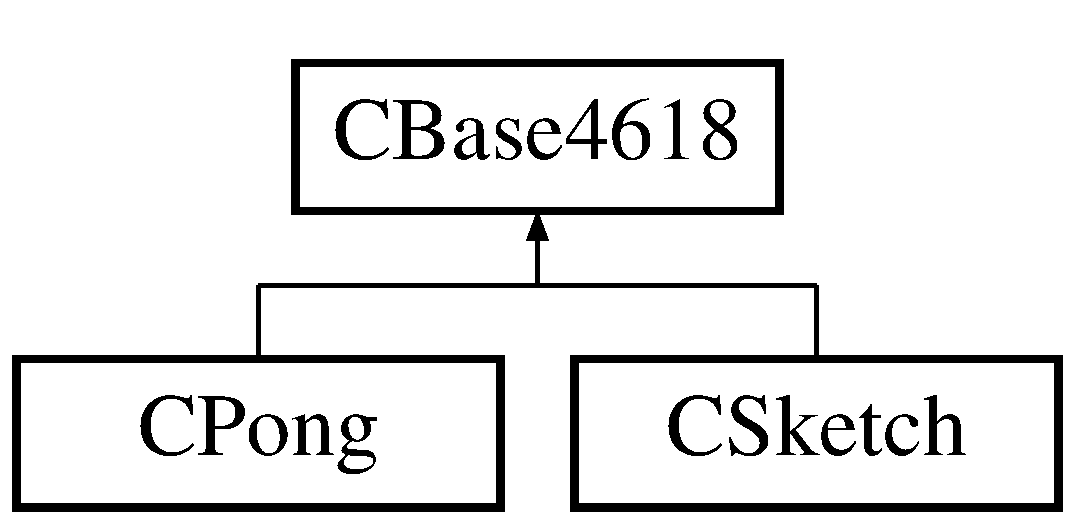
\includegraphics[height=2.000000cm]{class_c_base4618}
\end{center}
\end{figure}
\subsection*{Public Member Functions}
\begin{DoxyCompactItemize}
\item 
\hyperlink{class_c_base4618_a43202fe8782b8620c889b3d935759cdd}{C\+Base4618} (\hyperlink{class_c_control}{C\+Control} \+\_\+cctrl, cv\+::\+Mat \+\_\+canvas)
\item 
virtual void \hyperlink{class_c_base4618_a46e2ad109d3c7c877d00cff9093736c7}{update} (double \&, double \&)
\item 
virtual void \hyperlink{class_c_base4618_aa4e8190003db02c98e7e6bdcfdf0ee1a}{draw} (int, int)
\item 
void \hyperlink{class_c_base4618_a535e816d735d10d6048dd39cd893d393}{run} ()
\end{DoxyCompactItemize}
\subsection*{Protected Attributes}
\begin{DoxyCompactItemize}
\item 
\hypertarget{class_c_base4618_ae97e0017b88b5a71565e522ed0c04413}{}\label{class_c_base4618_ae97e0017b88b5a71565e522ed0c04413} 
\hyperlink{class_c_control}{C\+Control} {\bfseries \+\_\+cctrl}
\item 
\hypertarget{class_c_base4618_a1b925f757247b33ca2072f777f24582d}{}\label{class_c_base4618_a1b925f757247b33ca2072f777f24582d} 
cv\+::\+Mat {\bfseries \+\_\+canvas}
\end{DoxyCompactItemize}


\subsection{Detailed Description}
This class is a base class for future labs which contains functions and members that can be used by the derived class. 

\hyperlink{_c_base4618_8h_source}{C\+Base4618.\+h}

\begin{DoxyAuthor}{Author}
Jasdeep Grewal
\end{DoxyAuthor}
\begin{DoxyVersion}{Version}
1 -- 7 February 2019 
\end{DoxyVersion}


\subsection{Constructor \& Destructor Documentation}
\hypertarget{class_c_base4618_a43202fe8782b8620c889b3d935759cdd}{}\label{class_c_base4618_a43202fe8782b8620c889b3d935759cdd} 
\index{C\+Base4618@{C\+Base4618}!C\+Base4618@{C\+Base4618}}
\index{C\+Base4618@{C\+Base4618}!C\+Base4618@{C\+Base4618}}
\subsubsection{\texorpdfstring{C\+Base4618()}{CBase4618()}}
{\footnotesize\ttfamily C\+Base4618\+::\+C\+Base4618 (\begin{DoxyParamCaption}\item[{\hyperlink{class_c_control}{C\+Control}}]{\+\_\+cctrl,  }\item[{cv\+::\+Mat}]{\+\_\+canvas }\end{DoxyParamCaption})}

Creates contstructor for canvas and comport


\begin{DoxyParams}{Parameters}
{\em Canvas} & size is initialized \\
\hline
{\em Comport} & number is initailized\\
\hline
\end{DoxyParams}
\begin{DoxyReturn}{Returns}
Does not return anything 
\end{DoxyReturn}


\subsection{Member Function Documentation}
\hypertarget{class_c_base4618_aa4e8190003db02c98e7e6bdcfdf0ee1a}{}\label{class_c_base4618_aa4e8190003db02c98e7e6bdcfdf0ee1a} 
\index{C\+Base4618@{C\+Base4618}!draw@{draw}}
\index{draw@{draw}!C\+Base4618@{C\+Base4618}}
\subsubsection{\texorpdfstring{draw()}{draw()}}
{\footnotesize\ttfamily void C\+Base4618\+::draw (\begin{DoxyParamCaption}\item[{int}]{x,  }\item[{int}]{y }\end{DoxyParamCaption})\hspace{0.3cm}{\ttfamily [virtual]}}

Draws lines based on X and Y coordinates


\begin{DoxyParams}{Parameters}
{\em Repeatedly} & gets analog inputs and determines X and Y coordinates \\
\hline
{\em Makes} & a line using the X and Y coordinates\\
\hline
\end{DoxyParams}
\begin{DoxyReturn}{Returns}
Does not return anything 
\end{DoxyReturn}


Reimplemented in \hyperlink{class_c_pong_ac4687aab31fbe5912cac2058663163fa}{C\+Pong}, and \hyperlink{class_c_sketch_a9b5af655812ecfa15791f5199854a3a4}{C\+Sketch}.

\hypertarget{class_c_base4618_a535e816d735d10d6048dd39cd893d393}{}\label{class_c_base4618_a535e816d735d10d6048dd39cd893d393} 
\index{C\+Base4618@{C\+Base4618}!run@{run}}
\index{run@{run}!C\+Base4618@{C\+Base4618}}
\subsubsection{\texorpdfstring{run()}{run()}}
{\footnotesize\ttfamily void C\+Base4618\+::run (\begin{DoxyParamCaption}{ }\end{DoxyParamCaption})}

Runs the draw and update function


\begin{DoxyParams}{Parameters}
{\em Runs} & functions until q is pressed to quit\\
\hline
\end{DoxyParams}
\begin{DoxyReturn}{Returns}
Does not return anything 
\end{DoxyReturn}
\hypertarget{class_c_base4618_a46e2ad109d3c7c877d00cff9093736c7}{}\label{class_c_base4618_a46e2ad109d3c7c877d00cff9093736c7} 
\index{C\+Base4618@{C\+Base4618}!update@{update}}
\index{update@{update}!C\+Base4618@{C\+Base4618}}
\subsubsection{\texorpdfstring{update()}{update()}}
{\footnotesize\ttfamily void C\+Base4618\+::update (\begin{DoxyParamCaption}\item[{double \&}]{x\+Position,  }\item[{double \&}]{y\+Position }\end{DoxyParamCaption})\hspace{0.3cm}{\ttfamily [virtual]}}

Updates X and Y coordinates


\begin{DoxyParams}{Parameters}
{\em Gets} & analog inputs \\
\hline
{\em Updates} & them continuously to mimic an Etch-\/\+A-\/\+Sketch\\
\hline
\end{DoxyParams}
\begin{DoxyReturn}{Returns}
Does not return anything 
\end{DoxyReturn}


Reimplemented in \hyperlink{class_c_pong_a036cdd714486e765a658b835547d058e}{C\+Pong}, and \hyperlink{class_c_sketch_a81582a1c6eb7524db76546565412a88b}{C\+Sketch}.



The documentation for this class was generated from the following files\+:\begin{DoxyCompactItemize}
\item 
C\+Base4618.\+h\item 
C\+Base4618.\+cpp\end{DoxyCompactItemize}

\hypertarget{class_c_control}{}\section{C\+Control Class Reference}
\label{class_c_control}\index{C\+Control@{C\+Control}}


A control class that gets or sets the data by opening up a comport.  




{\ttfamily \#include $<$C\+Control.\+h$>$}

\subsection*{Public Member Functions}
\begin{DoxyCompactItemize}
\item 
\hypertarget{class_c_control_a3d1384d0e1ee2a4a478a798b46457468}{}\label{class_c_control_a3d1384d0e1ee2a4a478a798b46457468} 
void {\bfseries init\+\_\+com} (int comport)
\item 
bool \hyperlink{class_c_control_a0bad8e51e54cb6f1e2a7b51d3a3940d3}{get\+\_\+data} (int type, int channel, int \&result)
\item 
bool \hyperlink{class_c_control_a13f557815616ef66a8f5dd4b725d8c32}{set\+\_\+data} (int type, int channel, int val)
\item 
double \hyperlink{class_c_control_a0321002fa4b31b1e3da23a5f2f21ecc3}{get\+\_\+analog} (int)
\end{DoxyCompactItemize}


\subsection{Detailed Description}
A control class that gets or sets the data by opening up a comport. 

C\+Control.\+cpp

\begin{DoxyAuthor}{Author}
Jasdeep Grewal
\end{DoxyAuthor}
\begin{DoxyVersion}{Version}
1.\+0 -- 25 January 2019 
\end{DoxyVersion}


\subsection{Member Function Documentation}
\hypertarget{class_c_control_a0321002fa4b31b1e3da23a5f2f21ecc3}{}\label{class_c_control_a0321002fa4b31b1e3da23a5f2f21ecc3} 
\index{C\+Control@{C\+Control}!get\+\_\+analog@{get\+\_\+analog}}
\index{get\+\_\+analog@{get\+\_\+analog}!C\+Control@{C\+Control}}
\subsubsection{\texorpdfstring{get\+\_\+analog()}{get\_analog()}}
{\footnotesize\ttfamily double C\+Control\+::get\+\_\+analog (\begin{DoxyParamCaption}\item[{int}]{channel }\end{DoxyParamCaption})}

Sets data.


\begin{DoxyParams}{Parameters}
{\em Sets} & value of type, channel, and value\\
\hline
\end{DoxyParams}
\begin{DoxyReturn}{Returns}
Type, channel, and value if true 
\end{DoxyReturn}
\hypertarget{class_c_control_a0bad8e51e54cb6f1e2a7b51d3a3940d3}{}\label{class_c_control_a0bad8e51e54cb6f1e2a7b51d3a3940d3} 
\index{C\+Control@{C\+Control}!get\+\_\+data@{get\+\_\+data}}
\index{get\+\_\+data@{get\+\_\+data}!C\+Control@{C\+Control}}
\subsubsection{\texorpdfstring{get\+\_\+data()}{get\_data()}}
{\footnotesize\ttfamily bool C\+Control\+::get\+\_\+data (\begin{DoxyParamCaption}\item[{int}]{type,  }\item[{int}]{channel,  }\item[{int \&}]{result }\end{DoxyParamCaption})}

Gets a comport.


\begin{DoxyParams}{Parameters}
{\em opens} & comport\\
\hline
\end{DoxyParams}
\begin{DoxyReturn}{Returns}
Returns nothing 
\end{DoxyReturn}
\hypertarget{class_c_control_a13f557815616ef66a8f5dd4b725d8c32}{}\label{class_c_control_a13f557815616ef66a8f5dd4b725d8c32} 
\index{C\+Control@{C\+Control}!set\+\_\+data@{set\+\_\+data}}
\index{set\+\_\+data@{set\+\_\+data}!C\+Control@{C\+Control}}
\subsubsection{\texorpdfstring{set\+\_\+data()}{set\_data()}}
{\footnotesize\ttfamily bool C\+Control\+::set\+\_\+data (\begin{DoxyParamCaption}\item[{int}]{type,  }\item[{int}]{channel,  }\item[{int}]{val }\end{DoxyParamCaption})}

Gets data.


\begin{DoxyParams}{Parameters}
{\em Gets} & values from type, channel, and result\\
\hline
\end{DoxyParams}
\begin{DoxyReturn}{Returns}
Type, channel, and value if true 
\end{DoxyReturn}


The documentation for this class was generated from the following files\+:\begin{DoxyCompactItemize}
\item 
C\+Control.\+h\item 
C\+Control.\+cpp\end{DoxyCompactItemize}

\hypertarget{class_client}{}\section{Client Class Reference}
\label{class_client}\index{Client@{Client}}
\subsection*{Public Member Functions}
\begin{DoxyCompactItemize}
\item 
\hypertarget{class_client_ae48ea283b08db8a87601a96690895a21}{}\label{class_client_ae48ea283b08db8a87601a96690895a21} 
{\bfseries Client} (int port, std\+::string addr)
\item 
\hypertarget{class_client_a91961b4d21399184db9e8a15207a2597}{}\label{class_client_a91961b4d21399184db9e8a15207a2597} 
void {\bfseries tx\+\_\+str} (std\+::string str)
\item 
\hypertarget{class_client_a02fd5ad5279d63db63c9db4f199dc410}{}\label{class_client_a02fd5ad5279d63db63c9db4f199dc410} 
bool {\bfseries rx\+\_\+str} (std\+::string \&str)
\item 
\hypertarget{class_client_a34e7dbb4238cfdd8ce5aa705da011853}{}\label{class_client_a34e7dbb4238cfdd8ce5aa705da011853} 
bool {\bfseries rx\+\_\+im} (cv\+::\+Mat \&im)
\end{DoxyCompactItemize}


The documentation for this class was generated from the following files\+:\begin{DoxyCompactItemize}
\item 
Client.\+h\item 
Client.\+cpp\end{DoxyCompactItemize}

\hypertarget{class_c_pong}{}\section{C\+Pong Class Reference}
\label{class_c_pong}\index{C\+Pong@{C\+Pong}}


A class which is used to implement Pong.  




{\ttfamily \#include $<$C\+Pong.\+h$>$}

Inheritance diagram for C\+Pong\+:\begin{figure}[H]
\begin{center}
\leavevmode
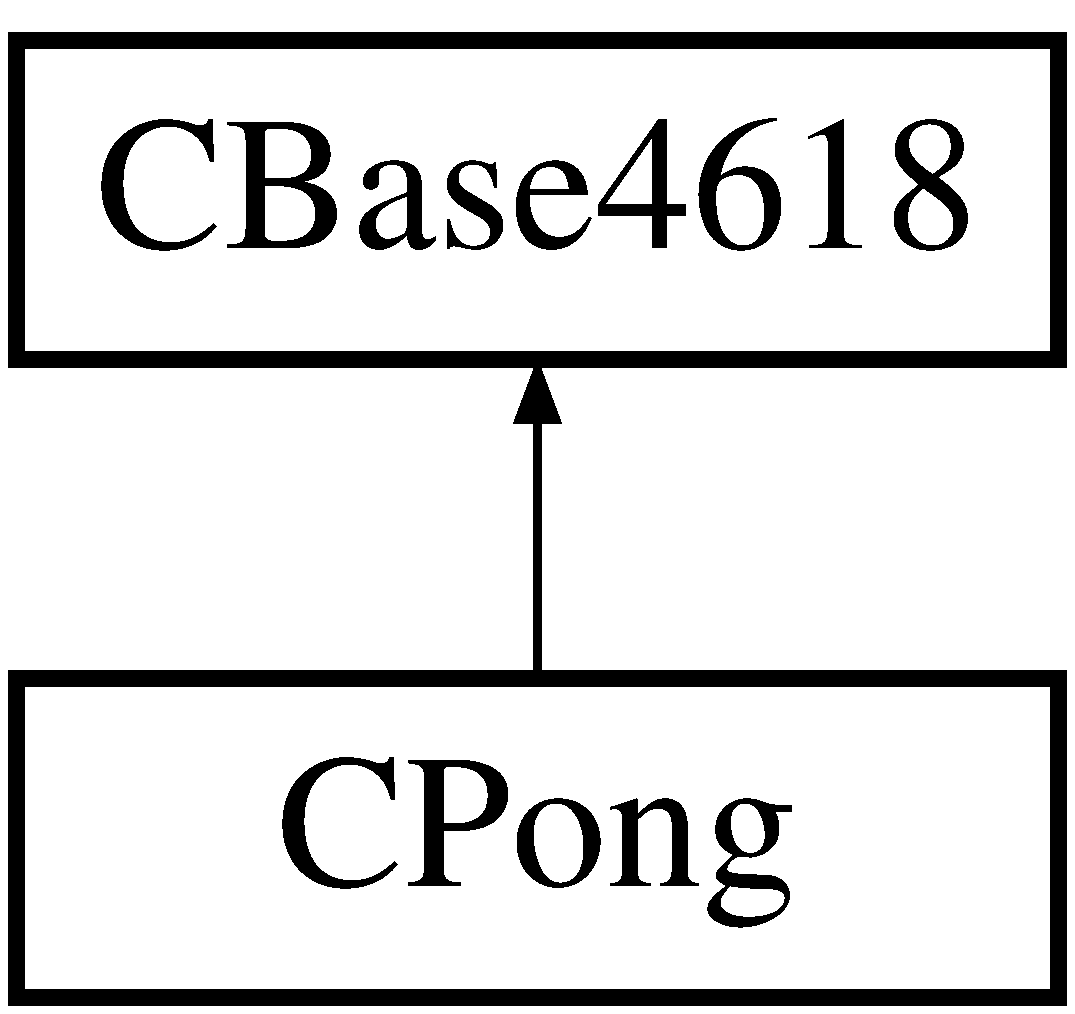
\includegraphics[height=2.000000cm]{class_c_pong}
\end{center}
\end{figure}
\subsection*{Public Member Functions}
\begin{DoxyCompactItemize}
\item 
\hyperlink{class_c_pong_a6eb8c1a5601f06350cc0c3d30fbc392a}{C\+Pong} (cv\+::\+Size, int)
\item 
void \hyperlink{class_c_pong_a036cdd714486e765a658b835547d058e}{update} (double \&x\+Position, double \&y\+Position)
\item 
void \hyperlink{class_c_pong_ac4687aab31fbe5912cac2058663163fa}{draw} (int x, int y)
\item 
bool \hyperlink{class_c_pong_a74d1c17870e642d1567833a9f40c870e}{btn\+Pressed} (int gpio\+Pin)
\end{DoxyCompactItemize}
\subsection*{Additional Inherited Members}


\subsection{Detailed Description}
A class which is used to implement Pong. 

\hyperlink{_c_pong_8h_source}{C\+Pong.\+h}

This class inherits from the base class called \hyperlink{_c_base4618_8h_source}{C\+Base4618.\+h} and overrides the functions.

\begin{DoxyAuthor}{Author}
Jasdeep Grewal
\end{DoxyAuthor}
\begin{DoxyVersion}{Version}
1 -- 8 February 2019 
\end{DoxyVersion}


\subsection{Constructor \& Destructor Documentation}
\hypertarget{class_c_pong_a6eb8c1a5601f06350cc0c3d30fbc392a}{}\label{class_c_pong_a6eb8c1a5601f06350cc0c3d30fbc392a} 
\index{C\+Pong@{C\+Pong}!C\+Pong@{C\+Pong}}
\index{C\+Pong@{C\+Pong}!C\+Pong@{C\+Pong}}
\subsubsection{\texorpdfstring{C\+Pong()}{CPong()}}
{\footnotesize\ttfamily C\+Pong\+::\+C\+Pong (\begin{DoxyParamCaption}\item[{cv\+::\+Size}]{\+\_\+canvas\+Size2,  }\item[{int}]{\+\_\+comport }\end{DoxyParamCaption})}

Creates constructor for canvas


\begin{DoxyParams}{Parameters}
{\em Canvas} & size is initialized \\
\hline
{\em Comport} & number is initialized\\
\hline
\end{DoxyParams}
\begin{DoxyReturn}{Returns}
Does not return anything 
\end{DoxyReturn}


\subsection{Member Function Documentation}
\hypertarget{class_c_pong_a74d1c17870e642d1567833a9f40c870e}{}\label{class_c_pong_a74d1c17870e642d1567833a9f40c870e} 
\index{C\+Pong@{C\+Pong}!btn\+Pressed@{btn\+Pressed}}
\index{btn\+Pressed@{btn\+Pressed}!C\+Pong@{C\+Pong}}
\subsubsection{\texorpdfstring{btn\+Pressed()}{btnPressed()}}
{\footnotesize\ttfamily bool C\+Pong\+::btn\+Pressed (\begin{DoxyParamCaption}\item[{int}]{gpio\+Pin }\end{DoxyParamCaption})}

Button debounce


\begin{DoxyParams}{Parameters}
{\em Uses} & number of ticks to debounce pushbutton\\
\hline
\end{DoxyParams}
\begin{DoxyReturn}{Returns}
True if button was pressed 
\end{DoxyReturn}
\hypertarget{class_c_pong_ac4687aab31fbe5912cac2058663163fa}{}\label{class_c_pong_ac4687aab31fbe5912cac2058663163fa} 
\index{C\+Pong@{C\+Pong}!draw@{draw}}
\index{draw@{draw}!C\+Pong@{C\+Pong}}
\subsubsection{\texorpdfstring{draw()}{draw()}}
{\footnotesize\ttfamily void C\+Pong\+::draw (\begin{DoxyParamCaption}\item[{int}]{x,  }\item[{int}]{y }\end{DoxyParamCaption})\hspace{0.3cm}{\ttfamily [virtual]}}

Moves paddle based on joystick position


\begin{DoxyParams}{Parameters}
{\em Repeatedly} & gets the analog input from the joystick \\
\hline
{\em Moves} & paddle using the analog input\\
\hline
\end{DoxyParams}
\begin{DoxyReturn}{Returns}
Does not return anything 
\end{DoxyReturn}


Reimplemented from \hyperlink{class_c_base4618_aa4e8190003db02c98e7e6bdcfdf0ee1a}{C\+Base4618}.

\hypertarget{class_c_pong_a036cdd714486e765a658b835547d058e}{}\label{class_c_pong_a036cdd714486e765a658b835547d058e} 
\index{C\+Pong@{C\+Pong}!update@{update}}
\index{update@{update}!C\+Pong@{C\+Pong}}
\subsubsection{\texorpdfstring{update()}{update()}}
{\footnotesize\ttfamily void C\+Pong\+::update (\begin{DoxyParamCaption}\item[{double \&}]{x\+Position,  }\item[{double \&}]{y\+Position }\end{DoxyParamCaption})\hspace{0.3cm}{\ttfamily [virtual]}}

Updates Y coordinates


\begin{DoxyParams}{Parameters}
{\em Gets} & analog inputs \\
\hline
{\em Updates} & joysyick position continuously to mimic an Etch-\/\+A-\/\+Sketch\\
\hline
\end{DoxyParams}
\begin{DoxyReturn}{Returns}
Does not return anything 
\end{DoxyReturn}


Reimplemented from \hyperlink{class_c_base4618_a46e2ad109d3c7c877d00cff9093736c7}{C\+Base4618}.



The documentation for this class was generated from the following files\+:\begin{DoxyCompactItemize}
\item 
C\+Pong.\+h\item 
C\+Pong.\+cpp\end{DoxyCompactItemize}

\hypertarget{class_c_sketch}{}\section{C\+Sketch Class Reference}
\label{class_c_sketch}\index{C\+Sketch@{C\+Sketch}}
Inheritance diagram for C\+Sketch\+:\begin{figure}[H]
\begin{center}
\leavevmode
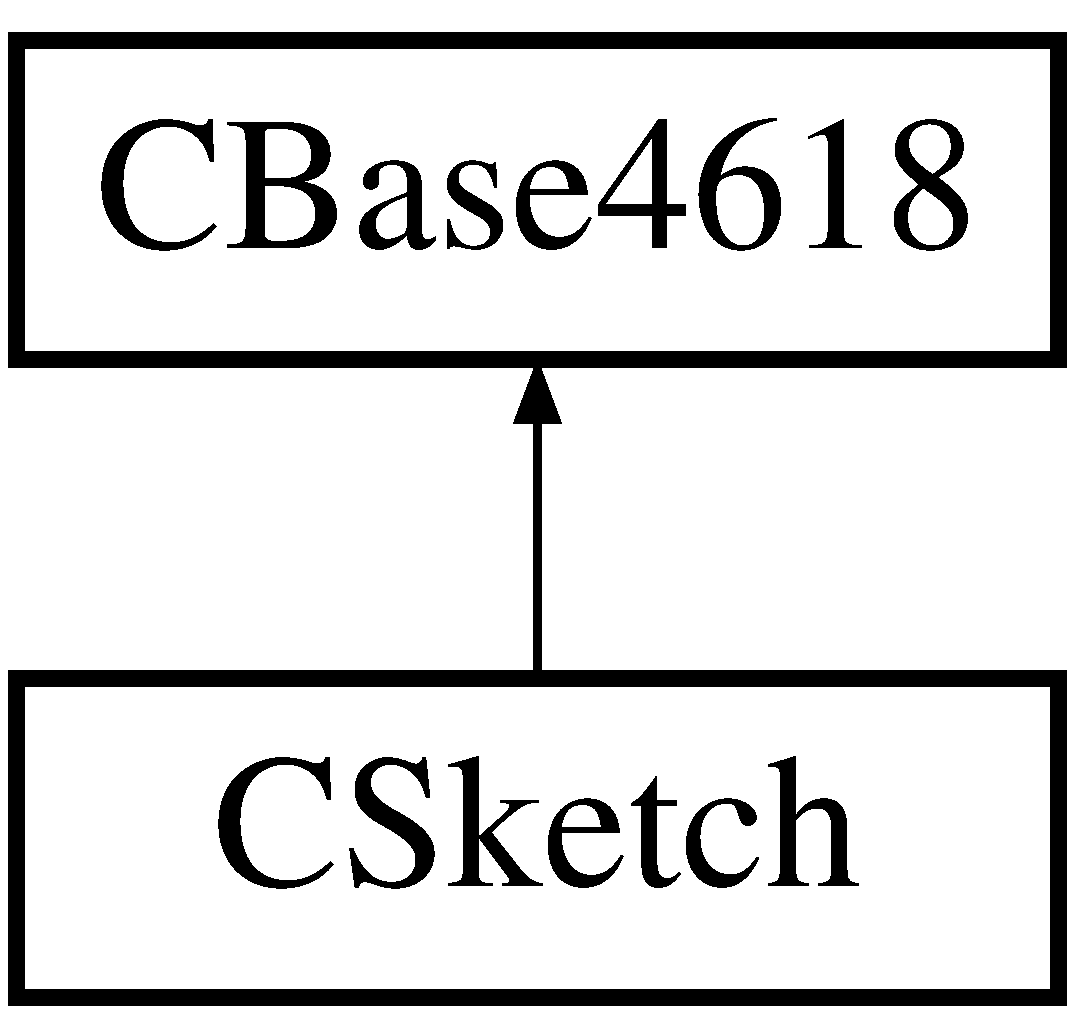
\includegraphics[height=2.000000cm]{class_c_sketch}
\end{center}
\end{figure}
\subsection*{Public Member Functions}
\begin{DoxyCompactItemize}
\item 
\hypertarget{class_c_sketch_aa426bb25ef429d04103b180863dbc11a}{}\label{class_c_sketch_aa426bb25ef429d04103b180863dbc11a} 
{\bfseries C\+Sketch} (cv\+::\+Size, int)
\item 
void \hyperlink{class_c_sketch_a81582a1c6eb7524db76546565412a88b}{update} (double \&x\+Position, double \&y\+Position)
\item 
void \hyperlink{class_c_sketch_a9b5af655812ecfa15791f5199854a3a4}{draw} (int x, int y)
\item 
\hypertarget{class_c_sketch_a9e73bdd4ab788236c1a682459d6a6075}{}\label{class_c_sketch_a9e73bdd4ab788236c1a682459d6a6075} 
bool {\bfseries btn\+Pressed} (int gpio\+Pin)
\end{DoxyCompactItemize}
\subsection*{Additional Inherited Members}


\subsection{Member Function Documentation}
\hypertarget{class_c_sketch_a9b5af655812ecfa15791f5199854a3a4}{}\label{class_c_sketch_a9b5af655812ecfa15791f5199854a3a4} 
\index{C\+Sketch@{C\+Sketch}!draw@{draw}}
\index{draw@{draw}!C\+Sketch@{C\+Sketch}}
\subsubsection{\texorpdfstring{draw()}{draw()}}
{\footnotesize\ttfamily void C\+Sketch\+::draw (\begin{DoxyParamCaption}\item[{int}]{x,  }\item[{int}]{y }\end{DoxyParamCaption})\hspace{0.3cm}{\ttfamily [virtual]}}

Draws lines based on X and Y coordinates


\begin{DoxyParams}{Parameters}
{\em Repeatedly} & gets analog inputs and determines X and Y coordinates \\
\hline
{\em Makes} & a line using the X and Y coordinates\\
\hline
\end{DoxyParams}
\begin{DoxyReturn}{Returns}
Does not return anything 
\end{DoxyReturn}


Reimplemented from \hyperlink{class_c_base4618_aa4e8190003db02c98e7e6bdcfdf0ee1a}{C\+Base4618}.

\hypertarget{class_c_sketch_a81582a1c6eb7524db76546565412a88b}{}\label{class_c_sketch_a81582a1c6eb7524db76546565412a88b} 
\index{C\+Sketch@{C\+Sketch}!update@{update}}
\index{update@{update}!C\+Sketch@{C\+Sketch}}
\subsubsection{\texorpdfstring{update()}{update()}}
{\footnotesize\ttfamily void C\+Sketch\+::update (\begin{DoxyParamCaption}\item[{double \&}]{x\+Position,  }\item[{double \&}]{y\+Position }\end{DoxyParamCaption})\hspace{0.3cm}{\ttfamily [virtual]}}

Updates X and Y coordinates


\begin{DoxyParams}{Parameters}
{\em Gets} & analog inputs \\
\hline
{\em Updates} & them continuously to mimic an Etch-\/\+A-\/\+Sketch\\
\hline
\end{DoxyParams}
\begin{DoxyReturn}{Returns}
Does not return anything 
\end{DoxyReturn}


Reimplemented from \hyperlink{class_c_base4618_a46e2ad109d3c7c877d00cff9093736c7}{C\+Base4618}.



The documentation for this class was generated from the following files\+:\begin{DoxyCompactItemize}
\item 
C\+Sketch.\+h\item 
C\+Sketch.\+cpp\end{DoxyCompactItemize}

\hypertarget{class_serial}{}\section{Serial Class Reference}
\label{class_serial}\index{Serial@{Serial}}
\subsection*{Public Member Functions}
\begin{DoxyCompactItemize}
\item 
\hypertarget{class_serial_a599d3e220888815b8da436ea45a5c655}{}\label{class_serial_a599d3e220888815b8da436ea45a5c655} 
bool {\bfseries open} (std\+::string comm\+Port\+Name, int bit\+Rate=115200)
\item 
int \hyperlink{class_serial_aae3d630a4fd81c8b148cb4eebdb91392}{write} (const char $\ast$buffer, int buff\+Len)
\item 
int \hyperlink{class_serial_a8266889eb5bfa7ef8b53595c5482133d}{read} (char $\ast$buffer, int buff\+Len)
\item 
\hypertarget{class_serial_a63b7abf172cad25bfc998b3b1f98310f}{}\label{class_serial_a63b7abf172cad25bfc998b3b1f98310f} 
void {\bfseries flush} ()
\end{DoxyCompactItemize}


\subsection{Member Function Documentation}
\hypertarget{class_serial_a8266889eb5bfa7ef8b53595c5482133d}{}\label{class_serial_a8266889eb5bfa7ef8b53595c5482133d} 
\index{Serial@{Serial}!read@{read}}
\index{read@{read}!Serial@{Serial}}
\subsubsection{\texorpdfstring{read()}{read()}}
{\footnotesize\ttfamily int Serial\+::read (\begin{DoxyParamCaption}\item[{char $\ast$}]{buffer,  }\item[{int}]{buff\+Len }\end{DoxyParamCaption})}

Reads a string of bytes from the serial port.


\begin{DoxyParams}{Parameters}
{\em buffer} & pointer to the buffer to be written to \\
\hline
{\em buff\+Len} & the size of the buffer\\
\hline
\end{DoxyParams}
\begin{DoxyReturn}{Returns}
int the number of bytes read 
\end{DoxyReturn}
\hypertarget{class_serial_aae3d630a4fd81c8b148cb4eebdb91392}{}\label{class_serial_aae3d630a4fd81c8b148cb4eebdb91392} 
\index{Serial@{Serial}!write@{write}}
\index{write@{write}!Serial@{Serial}}
\subsubsection{\texorpdfstring{write()}{write()}}
{\footnotesize\ttfamily int Serial\+::write (\begin{DoxyParamCaption}\item[{const char $\ast$}]{buffer,  }\item[{int}]{buff\+Len }\end{DoxyParamCaption})}

Writes a string of bytes to the serial port.


\begin{DoxyParams}{Parameters}
{\em buffer} & pointer to the buffer containing the bytes \\
\hline
{\em buff\+Len} & the number of bytes in the buffer\\
\hline
\end{DoxyParams}
\begin{DoxyReturn}{Returns}
int the number of bytes written 
\end{DoxyReturn}


The documentation for this class was generated from the following files\+:\begin{DoxyCompactItemize}
\item 
Serial.\+h\item 
Serial.\+cpp\end{DoxyCompactItemize}

\hypertarget{class_server}{}\section{Server Class Reference}
\label{class_server}\index{Server@{Server}}
\subsection*{Public Member Functions}
\begin{DoxyCompactItemize}
\item 
\hypertarget{class_server_a7ebba75484fe844bb3e2920205455a74}{}\label{class_server_a7ebba75484fe844bb3e2920205455a74} 
void {\bfseries start} (int port)
\item 
\hypertarget{class_server_ad49615121ae4496bb6f8248530937101}{}\label{class_server_ad49615121ae4496bb6f8248530937101} 
void {\bfseries set\+\_\+txim} (cv\+::\+Mat \&im)
\item 
\hypertarget{class_server_ad01a77ea78115b7e6fc0603e0f239963}{}\label{class_server_ad01a77ea78115b7e6fc0603e0f239963} 
void {\bfseries get\+\_\+cmd} (std\+::vector$<$ std\+::string $>$ \&cmds)
\end{DoxyCompactItemize}


The documentation for this class was generated from the following files\+:\begin{DoxyCompactItemize}
\item 
server.\+h\item 
server.\+cpp\end{DoxyCompactItemize}

%--- End generated contents ---

% Index
\backmatter
\newpage
\phantomsection
\clearemptydoublepage
\addcontentsline{toc}{chapter}{Index}
\printindex

\end{document}
